\documentclass[a4paper,fleqn,12pt]{cas-sc}

\usepackage[authoryear]{natbib}
\usepackage{tcolorbox}
\usepackage{graphicx}
\usepackage{textcomp}

\usepackage{amsfonts} % 显式加载字体
\DeclareMathAlphabet{\mathbb}{U}{msb}{m}{n}

\usepackage[linesnumbered, ruled]{algorithm2e}
\SetKwRepeat{Do}{do}{while}%
\newcommand\mycommfont[1]{\footnotesize\ttfamily\textcolor{blue}{#1}}
\SetCommentSty{mycommfont}

\usepackage{amssymb} % for empty set
\usepackage{booktabs}
\usepackage{tabularx}
\usepackage{array}
\usepackage{float}
\usepackage[flushleft]{threeparttable}
\usepackage{tabularray} % for better
\usepackage[subsection]{placeins}

\frenchspacing % for consistent spacing between sentences

\newcommand{\killpunct}[1]{} % for reference, remove the comma in the reference of Proceeding

\usepackage{caption}
\DeclareCaptionFont{singlespacing}{\singlespacing}
\captionsetup{font=singlespacing}

\usepackage{subcaption}

\usepackage{tabularray}

\usepackage{etoolbox}

% Modify font size of the bibliography
\apptocmd{\thebibliography}{\fontsize{10}{14}\selectfont}{}{}

\usepackage{capt-of}

\usepackage{lineno}

\usepackage{titlesec}
\titleformat*{\section}{\fontsize{12}{20}\selectfont\bfseries}

\usepackage{titlesec}
\titleformat*{\subsection}{\fontsize{12}{20}\selectfont\bfseries}

\SetKwInput{KwData}{Input}
\SetKwInput{KwResult}{Output}

\usepackage{diagbox}
\usepackage{url}
% centering figure and table captions

%%%Author macros
\def\tsc#1{\csdef{#1}{\textsc{\lowercase{#1}}\xspace}}
\tsc{WGM}
\tsc{QE}
\tsc{EP}
\tsc{PMS}
\tsc{BEC}
\tsc{DE}
%%%

\begin{document}
\let\WriteBookmarks\relax
\def\floatpagepagefraction{1}
\def\textpagefraction{.001}
% \shorttitle{Preprint submitted to \textit{Elsevier journal}}
% \shortauthors{Lei et~al.}
%\begin{frontmatter}

\title [mode = title]{Impact Evaluation of Transit Improvement Program: A Social Media Data Mining and Causal Inference Framework} 

% \author[1]{Da Lei}[%
% ]

% \address[1]{Department of Geography and Resource Management, The Chinese University of Hong Kong, Hong Kong, China}
% \address[2]{School of Humanities and Social Science, The Chinese University of Hong Kong, Shenzhen, China}


% \author[1]{Sylvia He}[\%
% ]
% \cormark[1]

% \author[2]{Shuli Luo}[\%
% ]

\cortext[cor1]{Corresponding author}


\begin{abstract}
Assessing the effectiveness of transit improvement programs is crucial to improving urban mobility, but traditional methods often lack timeliness and cannot capture passenger travel experiences. Although social media data can provide a wealth of real-time public opinions, there is a major research gap: Few studies have used these data to evaluate the impact of specific transit improvement programs by comparing passenger attitudes before and after implementation. To fill this gap, this paper proposes a new framework that combines advanced text mining with causal inference methods. Our approach uses semantic matching to associate unstructured social media posts with specific transit improvement programs and uses interruption time series analysis (ITSA) to quantify changes in passenger sentiment while controlling for potential time-trend effects. We apply the framework to a case study from Shenzhen Metro and analyze 88,253 Weibo posts to evaluate six different transit improvement programs. The results reveal substantial heterogeneity in program effectiveness: technology-oriented upgrades (information systems and payment methods) and affordability improvements demonstrated significant positive impacts with distinct temporal patterns, while a comfort-oriented intervention (temperature control) showed significant negative impacts, and amenity improvements had negligible effects. The study provides transit agencies with a reliable, data-based method to conduct evidence-based project assessments, distinguish between different impact trajectories, and better understand passenger travel experiences.
\end{abstract}

\begin{keywords}
 \sep social media data \sep transit improvement program impact evaluation \sep transit service quality
\end{keywords}


\maketitle
\setlength{\parindent}{15pt}
\setlength{\parskip}{0.1in}
\linenumbers

\section{Introduction}\label{sec:introduction}
Public transportation plays a vital role in urban mobility systems, providing essential services that can help to achieve the goals of sustainable development by reducing congestion, air pollution, and greenhouse gas emissions \citep{stjernborg2016role, mead2021road}. Despite these benefits, transit operators around the world continue to face continuing challenges to attract and retain passengers, especially when competing with private cars and emerging mobility services \citep{beirAo2007understanding}. To solve this problem, transit agencies continue to implement various transit improvement programs, covering aspects ranging from technology upgrades and infrastructure renovations to policy adjustments and customer service improvements \citep{luong2015public, fraser2024using}.

Assessing the effectiveness of these transit improvement programs is crucial to the strategic planning and operational management of the public transportation system. Traditional evaluation methods are heavily based on performance indicators such as passenger count, punctuality performance, and traveler satisfaction surveys \citep{nathanail2008measuring, eboli2011methodology}. Although these indicators can provide valuable information, they often fail to capture the nuanced views and real-time feedback of transit users \citep{collins2013social}. This limitation is prominent given that passenger perceptions and experiences directly influence their decisions to choose public transportation over other travel modes \citep{friman2001frequency, morton2016customer}.

With the proliferation of social media and the growing willingness of the public to share their experiences online, a large amount of user-generated content related to public transportation is available \citep{golder2011diurnal, kaplan2010users}. These data are an important resource for transit agencies trying to understand passenger sentiment and assess the impact of their transit improvement programs \citep{el2019linking, zhang2023changes}. Social media data has many advantages over traditional data sources. It provides real-time feedback, captures spontaneous and unfiltered opinions from users, and has the potential to reach a wider and more diverse audience than traditional surveys \citep{tasse2014using, haghighi2018using}.

Recent research has explored the potential of social media data in transportation planning and analysis. Studies have shown that Twitter data can be used to detect traffic incidents \citep{fu2015social}, analyze public perceptions of transit services \citep{luong2015public, collins2013social}, and evaluate the public response to transportation policies \citep{chakraborty2019public}. However, these studies typically focus on general sentiment analysis and do not link social media content to specific transit improvement programs or interventions \citep{ali2017fuzzy, ingvardson2019relationship}. Crucially, there is a lack of studies using social media data to evaluate specific transit improvement programs before and after their implementation, especially studies using causal inference methods to quantify the impacts \citep{mathur2021exploratory, liu2017monitoring}. This gap significantly limits the practical usefulness of social media analytics for evidence-based decision-making in transit agencies. Moreover, approaches to processing and analyzing social media data in transit evaluation remain underdeveloped, often relying on simplistic techniques that fail to capture contextual intricacies \citep{houston2015public, kamga2023utilizing}. Therefore, there is an urgent need for advanced frameworks to extract meaningful insights from unstructured social media posts and link them to specific transit improvement programs through causal analysis \citep{haghighi2018using}.

To address these limitations, this study proposes a novel framework, which combines advanced text mining techniques with causal inference methods, to evaluate the impact of transit improvement programs using social media data. The framework consists of three main components: (1) a text matching process aligns passenger feedback from social networks with specific transit improvement programs; (2) an Interrupted Time Series Analysis (ITSA) that quantifies changes in passenger sentiments before and after transit improvement program implementation; and (3) a set of statistical tests to assess the significance of transit improvement program impacts. The text matching process employs Latent Dirichlet Allocation (LDA) for topic modeling and Term Frequency-Inverse Document Frequency (TF-IDF) for feature extraction, followed by neural embeddings for semantic matching. This combination of techniques allows for the identification of relevant social media posts that reflect passenger experiences related to specific transit improvement programs, even when the posts do not explicitly mention program names or use standard terminology \citep{blei2003latent, lopez2016interrupted}. The ITSA method is suitable for evaluating the impact of interventions that have been implemented at clearly defined times \citep{wagner2002segmented, lopez2016interrupted}. By modeling passenger sentiment trends before and after transit improvement program implementation, ITSA can distinguish between short-term fluctuations and sustained sentiment trends, while controlling for confounding factors such as seasonal patterns and temporal autocorrelation \citep{schaffer2021interrupted, koppel2023disentangling}.

To validate our framework, we apply it to a case study of the Shenzhen Metro in China, using 88,253 Weibo posts collected from January 2019 to July 2023. The case study focuses on six transit improvement programs implemented by Shenzhen Metro during this period, covering different dimensions of transit service quality including comfort, convenience, affordability, information provision, and amenities. The results demonstrate the effectiveness of our approach in capturing heterogeneous impact patterns: three programs showed significant positive effects with distinct temporal profiles (immediate adoption, gradual improvement, and delayed appreciation), one program exhibited significant negative impacts despite addressing a common passenger concern, and two amenity-focused programs showed no detectable effects in general social media discourse. The contributions of this study are threefold. First, we develop a novel framework to bridge the gap between unstructured social media data and structured transit improvement program evaluation, enabling transit agencies to leverage the wealth of information available on social media platforms. Second, we demonstrate the application of ITSA in the context of transit improvement program evaluation, revealing how different intervention types produce distinct temporal impact patterns that simple before-after comparisons cannot capture. Third, we offer empirical evidence on the effectiveness of several transit improvement programs in Shenzhen Metro, providing actionable insights for transit agencies on which types of interventions generate widespread positive sentiment and which may require redesign.

The remainder of this paper is organized as follows. Section 2 reviews the relevant literature on the quality assessment of transit service, social media analytics in transportation, and causal inference methods for transit improvement program impact evaluation. Section 3 describes the methodology in detail, including the text matching process, ITSA model specification, and statistical testing procedures. Section 4 presents the case study of Shenzhen Metro, detailing the data collection, transit improvement program descriptions, and analysis results. Finally, Section 5 concludes with a discussion of the implications, limitations, and future directions of this research.

\section{Literature Review}\label{sec:liter}

\subsection{Causal Inference for Impact Evaluation in Transportation}
Establishing causal relationships between transportation interventions and observed outcomes represents a significant methodological challenge in transit improvement program evaluation \citep{karner2016transportation, hong2020causal}. Traditional before-after comparisons often fail to account for secular trends, seasonality, and confounding factors that can influence the observed changes independently of the intervention \citep{lechner2011estimation, imbens2015causal}.

Quasi-experimental designs have emerged as valuable approaches for strengthening causal inference in transit improvement program evaluation. Among these, interrupted time series (ITS) analysis has gained prominence as a robust method for assessing the impact of interventions when randomization is not feasible \citep{bernal2017interrupted, lopez2017interrupted}. The ITS approach examines the trajectory of an outcome measure before and after an intervention, accounting for pre-existing trends to isolate the effect of the intervention \citep{wagner2002segmented, bernal2016methodological}. \cite{kontopantelis2015regression} demonstrated the application of ITS analysis in evaluating policy interventions, highlighting its ability to control for time-varying confounders and detect both immediate and gradual effects. In the transportation context, \cite{morrison2018impact} employed ITS analysis to evaluate the impact of a new light rail line on traffic congestion, distinguishing the intervention effect from seasonal and long-term trends. Similarly, \cite{baek2016using} used this approach to assess the effectiveness of improved transit service to increase ridership, controlling for external factors such as fuel prices and economic conditions.

Advanced causal inference methods, such as difference-in-differences (DiD) and synthetic control methods, have also been applied in transit improvement program evaluation. \cite{hong2020causal} employed a DiD approach to evaluate the impact of transit-oriented development on travel behavior, comparing treated and control areas while accounting for time-invariant unobserved characteristics. \cite{zhang2021causal} developed a causal inference framework for assessing the vulnerability of urban metro systems, demonstrating the application of advanced methods to transportation infrastructure evaluation.

Despite these methodological advances, most traditional approaches to transit improvement program evaluation rely heavily on passenger satisfaction surveys and structured questionnaires. While these survey-based methods provide valuable insights, they suffer from several critical limitations that constrain their utility for timely and comprehensive program assessment. \cite{carrel2019survey} identified systematic biases in survey-based measurements of transit customer loyalty, finding that self-reported data frequently overestimates actual transit usage and fails to capture temporal variations in behavior. \cite{echaniz2020modelling} demonstrated that missing information and respondent non-response in satisfaction surveys can significantly bias model estimates and lead to incorrect policy conclusions. Furthermore, traditional surveys are characterized by high data collection costs, significant time lags between data gathering and analysis, and survey fatigue among respondents that reduces response rates and data quality \citep{roberts2021doing, tyrinopoulos2008public}. These limitations highlight the need for complementary data sources that can capture passenger experiences more comprehensively and in real-time.

\subsection{Social Media Data in Transit Service Evaluation}

The emergence of social media platforms has created new opportunities for understanding passenger experiences and evaluating transit service quality. As an increasingly prominent data source, social media offers several advantages over traditional survey methods: it captures spontaneous, unsolicited feedback in real-time, provides access to larger and more diverse samples of transit users, and enables continuous monitoring of public sentiment without the costs and delays associated with structured surveys \citep{nikolaidou2018utilizing}. These characteristics have motivated a growing body of research exploring the potential of social media data for transit service evaluation and performance monitoring.

Recent studies have demonstrated the feasibility of mining social media platforms, particularly Twitter and Weibo, to assess various dimensions of transit service quality. \cite{haghighi2018using} developed a framework for evaluating transit riders' opinions about service quality from Twitter data, demonstrating that social media sentiment correlates with traditional satisfaction measures while providing more granular temporal resolution. \cite{collins2013social} introduced a novel transit rider satisfaction metric based on social media sentiment analysis, showing that online discussions reflect passenger experiences across multiple service dimensions including reliability, comfort, and safety. Beyond general service evaluation, researchers have employed text mining and sentiment analysis techniques to monitor transit system performance and detect service problems \citep{li2019mining, gong2024framework}. More recent work has begun examining how passengers respond to specific service changes through social media discourse \citep{alsahar2024using}.

However, the existing literature predominantly focuses on using social media data to evaluate the current state or ongoing performance of transit systems, rather than assessing the causal impacts of specific improvement interventions. While these studies have established the value of social media as a data source for understanding passenger sentiment, they typically employ descriptive analytics or correlational approaches that cannot distinguish between program effects and confounding temporal trends. Critically absent from the literature are rigorous quasi-experimental evaluations that leverage social media data to quantify how specific transit improvement programs influence passenger experiences before and after implementation. This gap is particularly significant given the increasing investments transit agencies make in service improvements and their need for evidence-based assessment of program effectiveness.

\section{Methodology}\label{sec:Methodology}

This section presents our methodological framework for evaluating transit improvement programs using social media data. The framework integrates advanced natural language processing (NLP) techniques with robust causal inference methods to systematically analyze how transit improvement programs influence passenger sentiment. As illustrated in \hyperref[fig:methodology_framework]{Fig.~\ref{fig:methodology_framework}}, our approach consists of three main components: (1) data preprocessing and semantic matching, (2) sentiment analysis and aggregation, and (3) impact evaluation using interrupted time series analysis.

\begin{figure}[htbp]
\centering
\includegraphics[width=0.9\textwidth]{figs/methodological framework.pdf}
\caption{Data Preprocessing and Transit Improvement Program Matching}
\label{fig:methodology_framework}
\end{figure}

\subsection{Data Preprocessing and Semantic Matching}

\subsubsection{Latent Dirichlet Allocation for Topic Discovery}

The first step in our framework involves processing unstructured social media posts to identify latent themes relevant to transit improvement programs. We employ Latent Dirichlet Allocation (LDA) \citep{blei2003latent}, a probabilistic topic modeling technique that discovers hidden thematic structures within text data. LDA models each document as a mixture of topics, where each topic is characterized by a distribution over words.

For preprocessing, we first remove URLs, special characters, and numbers from the text, then segment Chinese text using Jieba,\footnote{Jieba: \url{https://github.com/fxsjy/jieba}} a widely-used open-source Chinese text segmentation library. We eliminate stopwords and short words (typically single characters), as they convey minimal semantic meaning. To improve the segmentation quality for transit-specific content, we augment the Jieba dictionary with domain-relevant terms such as metro station names.

The LDA model is formally defined as:

\begin{align}
p(\theta, \mathbf{z}, \mathbf{w} | \alpha, \beta) = p(\theta | \alpha) \prod_{n=1}^{N} p(z_n | \theta) p(w_n | z_n, \beta)
\end{align}

where $\theta$ represents the document-topic distribution, $\mathbf{z}$ denotes the topic assignments, $\mathbf{w}$ represents the observed words, and $\alpha$ and $\beta$ are the hyperparameters for the Dirichlet priors on the document-topic and topic-word distributions, respectively.

To enhance model robustness, we optimize the LDA hyperparameters through multiple initializations with different random seeds, selecting the model with the lowest perplexity score. For our implementation, we set the number of topics $K = 15$, document-topic prior $\alpha = 0.05$, and topic-word prior $\beta = 0.005$, which we determined through empirical testing to provide interpretable topics while maintaining adequate discrimination between service quality dimensions.

\subsubsection{TF-IDF Feature Extraction}

After topic modeling, we employ Term Frequency-Inverse Document Frequency (TF-IDF) transformation to identify the most distinctive terms for each topic. The TF-IDF score for a term $t$ in document $d$ within corpus $D$ is computed as:

\begin{align}
\text{TF-IDF}(t, d, D) = \text{TF}(t, d) \times \text{IDF}(t, D)
\end{align}

where $\text{TF}(t, d)$ is the frequency of term $t$ in document $d$, and $\text{IDF}(t, D)$ is calculated as:

\begin{align}
\text{IDF}(t, D) = \log\frac{|D|}{|\{d \in D: t \in d\}|}
\end{align}

This transformation assigns higher weights to terms that are frequent in a specific document but rare across the corpus, which helps identify the most characteristic words for each topic. We apply TF-IDF transformation to the word-document matrix before fitting the LDA model, which helps improve topic coherence and interpretability.

\subsubsection{Neural Embedding for Semantic Matching}

To connect passenger feedback with specific transit improvement programs, we implement a semantic matching approach using neural embeddings. Specifically, we utilize the multilingual MiniLM-L12-v2 model from the sentence-transformers framework \citep{reimers2019sentence}, which maps text into a dense 384-dimensional vector space where semantically similar texts have high cosine similarity.

For each transit improvement program, we create a document that describes its objectives and features, then compute the embedding vector for this description. Similarly, we compute embedding vectors for each processed social media post. The semantic similarity between a transit improvement program $p$ and a post $s$ is calculated as:

\begin{align}
\text{sim}(p, s) = \frac{\mathbf{v}_p \cdot \mathbf{v}_s}{||\mathbf{v}_p|| \cdot ||\mathbf{v}_s||}
\end{align}

where $\mathbf{v}_p$ and $\mathbf{v}_s$ are the embedding vectors for the transit improvement program description and social media post, respectively. We establish a similarity threshold based on empirical testing, which balances precision and recall in matching relevant posts to transit improvement programs. Posts exceeding this threshold are considered relevant to the corresponding transit improvement program and included in the subsequent analysis.

\subsection{Sentiment Analysis and Aggregation}

\subsubsection{Sentiment Analysis Approach}

Given the specificity of transit-related terminology and the Chinese language context, we employ a domain-adapted sentiment analysis approach that combines a pre-trained sentiment model with domain-specific adjustments. For each post $s$, we compute a sentiment score $f(s) \in [-1, 1]$, where $-1$ represents extremely negative sentiment, $0$ represents neutral sentiment, and $1$ represents extremely positive sentiment. The sentiment score is computed as:

\begin{align}
f(s) = \text{clip}\left( \alpha \cdot f_{\text{base}}(s) + \beta \cdot f_{\text{lex}}(s) \right)
\end{align}

where $f_{\text{base}}(s)$ denotes the base sentiment score from a pre-trained model (e.g., BERT), $f_{\text{lex}}(s)$ represents the domain-adapted score from our transit-specific lexicon, $\alpha$ and $\beta$ are weighting coefficients ($\alpha + \beta = 1$) that balance model prediction and domain knowledge, and $\text{clip}(x) = \max(-1, \min(1, x))$ ensures scores stay within $[-1, 1]$.

The domain-adapted score $f_{\text{lex}}(s)$ accounts for negation patterns and intensifiers:
\begin{align}
f_{\text{lex}}(s) = \frac{1}{|s|} \sum_{w_i \in s} \gamma_i \cdot \text{sign}_i \cdot d(w_i)
\end{align}

where $d(w_i)$ is the sentiment polarity of word $w_i$ in our domain lexicon ($d(w_i) \in [-1, 1]$), $\text{sign}_i = (-1)^{n_i}$ handles negation patterns with $n_i$ counting negation words preceding $w_i$, $\gamma_i$ is the intensification factor (1.5 for strong intensifiers, 1.2 for medium intensifiers, and 1.0 otherwise), and $|s|$ is the post length in tokens.

This formulation integrates state-of-the-art deep learning with domain-specific linguistic rules to accurately capture passenger sentiment in the transit context.

\subsection{Impact Evaluation Using Interrupted Time Series Analysis}

\subsubsection{Model Specification}

To quantify the impact of transit improvement programs on passenger sentiment, we employ ITSA, a quasi-experimental design that evaluates interventions by examining changes in time series data patterns before and after implementation \citep{bernal2017interrupted}. ITSA is well-suited for our context as it can distinguish between immediate and gradual effects while controlling for pre-existing trends.

Our core ITSA model specification is:

\begin{align}
Y_t = \beta_0 + \beta_1 T_t + \beta_2 X_t + \beta_3 X_t T_t + \epsilon_t
\end{align}

where $Y_t$ represents the mean sentiment score at time $t$, $T_t$ indicates the time elapsed since the start of the study, $X_t$ is a dummy variable that distinguishes between pre-intervention ($X_t = 0$) and post-intervention periods ($X_t = 1$), $X_t T_t$ serves as an interaction term measuring time since the intervention occurred, and $\epsilon_t$ denotes the error term.

In this model, $\beta_0$ represents the baseline level, $\beta_1$ captures the pre-intervention trend, $\beta_2$ indicates the immediate change in level following intervention, and $\beta_3$ represents the change in trend after intervention.

\subsubsection{Addressing Time Series Complexities}

To handle the complexities inherent in time series data, we extend the basic ITSA model to account for:

\textbf{Autocorrelation:} We test for autocorrelation in the residuals using the Durbin-Watson statistic and incorporate autoregressive (AR) terms when necessary:

\begin{align}
Y_t = \beta_0 + \beta_1 T_t + \beta_2 X_t + \beta_3 X_t T_t + \sum_{i=1}^{p} \phi_i Y_{t-i} + \epsilon_t
\end{align}

where $p$ is the order of the autoregressive process, and $\phi_i$ are the AR coefficients.

\textbf{Seasonal Patterns:} We incorporate seasonal components to account for cyclical variations in transit usage and social media activity:

\begin{align}
Y_t = \beta_0 + \beta_1 T_t + \beta_2 X_t + \beta_3 X_t T_t + \sum_{j=1}^{J} \gamma_j S_{j,t} + \epsilon_t
\end{align}

where $S_{j,t}$ are seasonal indicator variables, and $\gamma_j$ are the corresponding coefficients.

\textbf{Heteroskedasticity:} We implement robust standard errors to address potential heteroskedasticity in the variance of the error terms.

\subsubsection{Placebo Tests and Robustness Checks}

To strengthen causal inference, we conduct several robustness checks: performing placebo tests by artificially shifting the intervention point to different time periods (expecting the strongest effect at the true intervention point); controlling for variation in the number of social media posts across time periods by including sample size as a covariate; and testing alternative model specifications by varying parameters such as aggregation periods, semantic matching thresholds, and sentiment analysis approaches.


\section{Case study}\label{sec:CaseStudy}

\subsection{Overview of Shenzhen Metro System}

Shenzhen Metro, operated by Shenzhen Metro Group Co., Ltd., serves as the primary rapid transit system for Shenzhen, one of China's major metropolitan areas in Guangdong Province. Since its first line opened in 2004, the system has expanded significantly to accommodate the city's rapid growth and development. As of 2023, the network comprises 16 operational lines spanning approximately 530 kilometers with 345 stations, making it one of the largest and busiest metro systems in China \citep{he2019geographically}. The system serves a diverse population of over 13 million residents and handles an average daily ridership exceeding 7 million passengers \citep{li2022comparative}. As a technology hub often referred to as "China's Silicon Valley," Shenzhen has integrated numerous technological innovations into its metro operations, including digital payment systems, facial recognition technology, and AI-powered crowd management systems \citep{guo2019smart}. Shenzhen Metro has implemented various transit improvement programs in recent years aimed at enhancing passenger experience across multiple dimensions of service quality. These improvements include technological innovations, infrastructure upgrades, policy changes, and customer service enhancements \citep{deng2021quality}. The evaluation of these transit improvement programs presents an ideal context for applying our proposed framework, as it allows us to investigate how different types of service improvements affect passenger sentiment and experience.

\subsection{Data Collection and Processing}

\subsubsection{Social Media Data Source}

For our analysis, we collected 88,253 Weibo posts related to Shenzhen Metro services between January 2019 and July 2023. Weibo, often described as China's equivalent to Twitter, serves as a major platform for public expression and opinion sharing in China, with approximately 530 million monthly active users as of 2022 \citep{wang2022empirical}. This platform offers several advantages for transit improvement program evaluation: it captures spontaneous, real-time passenger feedback outside the constraints of structured surveys, provides access to a larger and potentially more diverse sample of transit users, allows for the analysis of temporal patterns in public sentiment before and after transit improvement program implementation, and contains rich contextual information, including user characteristics and interaction patterns.

The data collection process involved an API-based retrieval using keywords related to Shenzhen Metro, including the system's name in different variations (e.g., "Shenzhen Metro", "Shenzhen Subway") and station names. We implemented comprehensive error handling and rate limiting to comply with platform policies while maximizing data quality.

\subsection{Transit Improvement Programs}

Our case study focused on six transit improvement programs implemented by Shenzhen Metro between 2020 and 2023. These transit improvement programs span different dimensions of transit service quality, including comfort, technology, convenience, affordability, and accessibility. \hyperref[tab:transit_improvement_programs]{Table~\ref{tab:transit_improvement_programs}} provides an overview of these transit improvement programs. Each transit improvement program represents a distinct approach to service improvement.

\begin{table}[h]
\centering
\caption{Transit Improvement Programs}
\label{tab:transit_improvement_programs} % transit improvement program table label
\begin{tabular}{|l|p{5cm}|p{2cm}|p{2cm}|}
\hline
\textbf{Name} & \textbf{Description} & \textbf{Service Dimension} & \textbf{Implementation Date} \\
\hline
Temperature & Different temperatures in the same carriage & Comfort & August 2022 \\
\hline
Smart Map Display & Enhanced passenger information through dynamic digital maps that update in real-time to show train location, estimated arrival times, and transfer information. & Information & October 2021 \\
\hline
QR Code Payment & Introduced contactless QR code payment options, reducing reliance on physical cards and expanding payment flexibility. & Convenience & March 2020 \\
\hline
Restroom Renovation & Improved station amenities through comprehensive renovation of restroom facilities at 82 stations across the network. & Amenities & June 2021 \\
\hline
Mobile Nursing Rooms & Enhanced accessibility for caregivers by installing mobile nursing room facilities at strategic locations throughout the network. & Accessibility & September 2022 \\
\hline
Fare Reduction & Increased affordability through a targeted fare reduction plan, particularly for commuters and frequent riders. & Affordability & January 2023 \\
\hline
\end{tabular}
\end{table}

\subsubsection{Data Preprocessing and Transit Improvement Program Matching}

The collected Weibo posts underwent several preprocessing steps before being matched to specific transit improvement programs, as illustrated in \hyperref[fig:match_workflow]{Fig.~\ref{fig:match_workflow}}. First, we removed URLs, special characters, and numbers from the text and segmented Chinese text using Jieba, a widely-used open-source Chinese text segmentation library. To improve segmentation quality for transit-specific content, we augmented the dictionary with domain-relevant terms such as metro station names. Following text cleaning, we applied Latent Dirichlet Allocation (LDA) to identify latent thematic structures within the corpus. The LDA model was optimized with a topic count of $K = 15$, document-topic prior $\alpha = 0.05$, and topic-word prior $\beta = 0.005$, determined through empirical testing to provide interpretable topics while maintaining adequate discrimination between service quality dimensions. To enhance topic coherence and interpretability, we employed Term Frequency-Inverse Document Frequency (TF-IDF) transformation, which assigns higher weights to terms that are frequent in specific documents but rare across the corpus.

\begin{figure}[htbp]
\centering
\includegraphics[width=0.8\textwidth]{figs/Data Preprocessing and Program Matching Workflow.pdf} % transit improvement program workflow figure
\caption{Data Preprocessing and Transit Improvement Program Matching}
\label{fig:match_workflow}
\end{figure}

The critical step in our methodology involved establishing semantic connections between passenger feedback and specific transit improvement programs. We utilized the multilingual MiniLM-L12-v2 model from the sentence-transformers framework \citep{reimers2019sentence}, which maps text into a dense 384-dimensional vector space. This approach enabled us to calculate semantic similarity scores between transit improvement program descriptions and social media posts, addressing the fundamental challenge of automatically identifying which posts relate to specific service improvements. To determine the optimal similarity threshold for matching, we conducted a systematic evaluation across seven threshold values: 0.25, 0.35, 0.45, 0.55, 0.65, 0.75, and 0.85. Two domain experts independently validated a randomly selected subset of 500 matches at each threshold level, assessing the semantic relevance between matched posts and transit improvement programs. As shown in \hyperref[fig:threshold_tradeoff_analysis]{Fig.~\ref{fig:threshold_tradeoff_analysis}}, higher similarity thresholds yielded improved matching accuracy, ranging from 72.3\% at threshold 0.25 to 96.8\% at threshold 0.85. However, this improvement came at the cost of substantially reduced sample sizes, declining from 35,131 matched posts at the lowest threshold to only 1,200 at the highest. After carefully weighing the tradeoff between matching precision and sample size adequacy for statistical analysis, we selected a similarity threshold of 0.55, which achieved 87.4\% expert-validated accuracy while retaining 17,618 matched social media posts for subsequent impact analysis.

\begin{figure}[htbp]
\centering
\includegraphics[width=0.99\textwidth]{figs/threshold_tradeoff_analysis.pdf}
\caption{Tradeoff Analysis Between Matching Accuracy and Sample Size Across Similarity Thresholds}
\label{fig:threshold_tradeoff_analysis}
\end{figure}

\subsection{Preliminary Statistical Analysis}

Before implementing the more sophisticated Interrupted Time Series Analysis, we conducted basic statistical tests to examine overall patterns in passenger sentiment before and after transit improvement program implementation. Although these preliminary analyses provide initial insights, they reveal important limitations that necessitate more robust analytical approaches.

\hyperref[fig:sentiment_distribution]{Fig.~\ref{fig:sentiment_distribution}} illustrates the distribution of sentiment scores between the six transit improvement programs, comparing the pre- and post-implementation periods. The visualization reveals heterogeneous patterns across different transit improvement programs. Technology-oriented transit improvement programs (Smart Map Display and QR Code Payment) show predominantly negative sentiment in the pre-implementation period, suggesting existing passenger dissatisfaction with these service aspects that the interventions aimed to address. Both programs exhibit shifts toward more positive sentiment post-implementation, with QR Code Payment showing a more pronounced shift consistent with its significant immediate level change. In contrast, the Fare Reduction transit improvement program exhibits moderately positive sentiment even before implementation, with a complex distributional pattern post-implementation that reflects the "initial disappointment followed by growing appreciation" dynamic. Most notably, the Temperature program shows a clear shift toward more negative sentiment post-implementation, consistent with the intervention's adverse effects revealed in time series analysis. The Mobile Nursing Rooms and Restroom Renovation programs show high baseline sentiment with minimal distributional changes, reflecting their limited impact on general passenger discourse.

\begin{figure}[htbp]
\centering
\includegraphics[width=0.99\textwidth]{figs/sentiment_distribution.pdf}
\caption{Sentiment Distribution by Transit Improvement Program Before and After Implementation}
\label{fig:sentiment_distribution}
\end{figure}

\hyperref[tab:basic_stats]{Table~\ref{tab:basic_stats}} presents the results of the paired t-test examining changes in the mean sentiment scores. Four transit improvement programs demonstrate statistically significant changes: Smart Map Display (t=13.50, p<0.001), QR Code Payment (t=15.85, p<0.001), Fare Reduction (t=13.15, p<0.001), and Temperature (t=-28.37, p<0.001). The technology-oriented programs (Smart Map Display and QR Code Payment) both show positive sentiment changes with comparable magnitudes (0.090 and 0.082 respectively), though subsequent time series analysis reveals distinct temporal patterns underlying these aggregate measures. The Temperature transit improvement program shows a substantial negative change (-0.219), the largest absolute change among all programs, suggesting significant sentiment deterioration following implementation. Interestingly, the Fare Reduction program shows a positive overall change (0.053), though this aggregate measure masks the complex temporal dynamics revealed in subsequent ITSA.

\begin{table}[htbp]
\centering
\caption{T-test results for passenger sentiment analysis}
\label{tab:basic_stats}
\begin{tabular}{lccccc}
\hline
Transit Improvement Program & Pre-Mean & Post-Mean & Mean Diff. & t-statistic & p-value \\
\hline
Smart Map Display & -0.213 & -0.123 & 0.090 & 13.50 & <0.001*** \\
QR Code Payment & -0.215 & -0.133 & 0.082 & 15.85 & <0.001*** \\
Fare Reduction & 0.188 & 0.241 & 0.053 & 13.15 & <0.001*** \\
Temperature & 0.130 & -0.088 & -0.219 & -28.37 & <0.001*** \\
Mobile Nursing Rooms & 0.682 & 0.664 & -0.018 & -1.32 & 0.186 \\
Restroom Renovation & 0.397 & 0.357 & -0.039 & -0.85 & 0.394 \\
\hline
\multicolumn{6}{l}{\footnotesize{*** p < 0.001}}
\end{tabular}
\end{table}

Chi-square tests examining the association between implementation periods and sentiment categories yield contradictory results (\hyperref[tab:categorical_tests]{Table~\ref{tab:categorical_tests}}). All transit improvement programs show statistically significant associations (p<0.001), including Mobile Nursing Rooms and Restroom Renovation, which demonstrated non-significant results in the t-tests. This inconsistency highlights a fundamental limitation of these basic approaches when applied to complex time series data.

\begin{table}[htbp]
\centering
\caption{Chi-square test results for passenger sentiment analysis}
\label{tab:categorical_tests}
\begin{tabular}{lcc}
\hline
Transit Improvement Program & Chi-square & p-value \\
\hline
Smart Map Display & 112.71 & <0.001*** \\
QR Code Payment & 142.87 & <0.001*** \\
Fare Reduction & 89.45 & <0.001*** \\
Temperature & 156.23 & <0.001*** \\
Mobile Nursing Rooms & 45.67 & <0.001*** \\
Restroom Renovation & 78.34 & <0.001*** \\
\hline
\multicolumn{3}{l}{\footnotesize{*** p < 0.001}}
\end{tabular}
\end{table}

The temporal visualization of aggregated sentiment data (\hyperref[fig:tsa_time_series]{Fig.~\ref{fig:tsa_time_series}}) reveals complex patterns that simple before-after comparisons cannot adequately capture. These plots demonstrate substantial variability over time, with apparent seasonal fluctuations and trend changes that occur independently of transit improvement program implementation dates. Such patterns suggest that observed differences between pre- and post-implementation periods may be confounded by underlying temporal trends rather than representing true transit improvement program effects.

\begin{figure}[htbp]
\centering
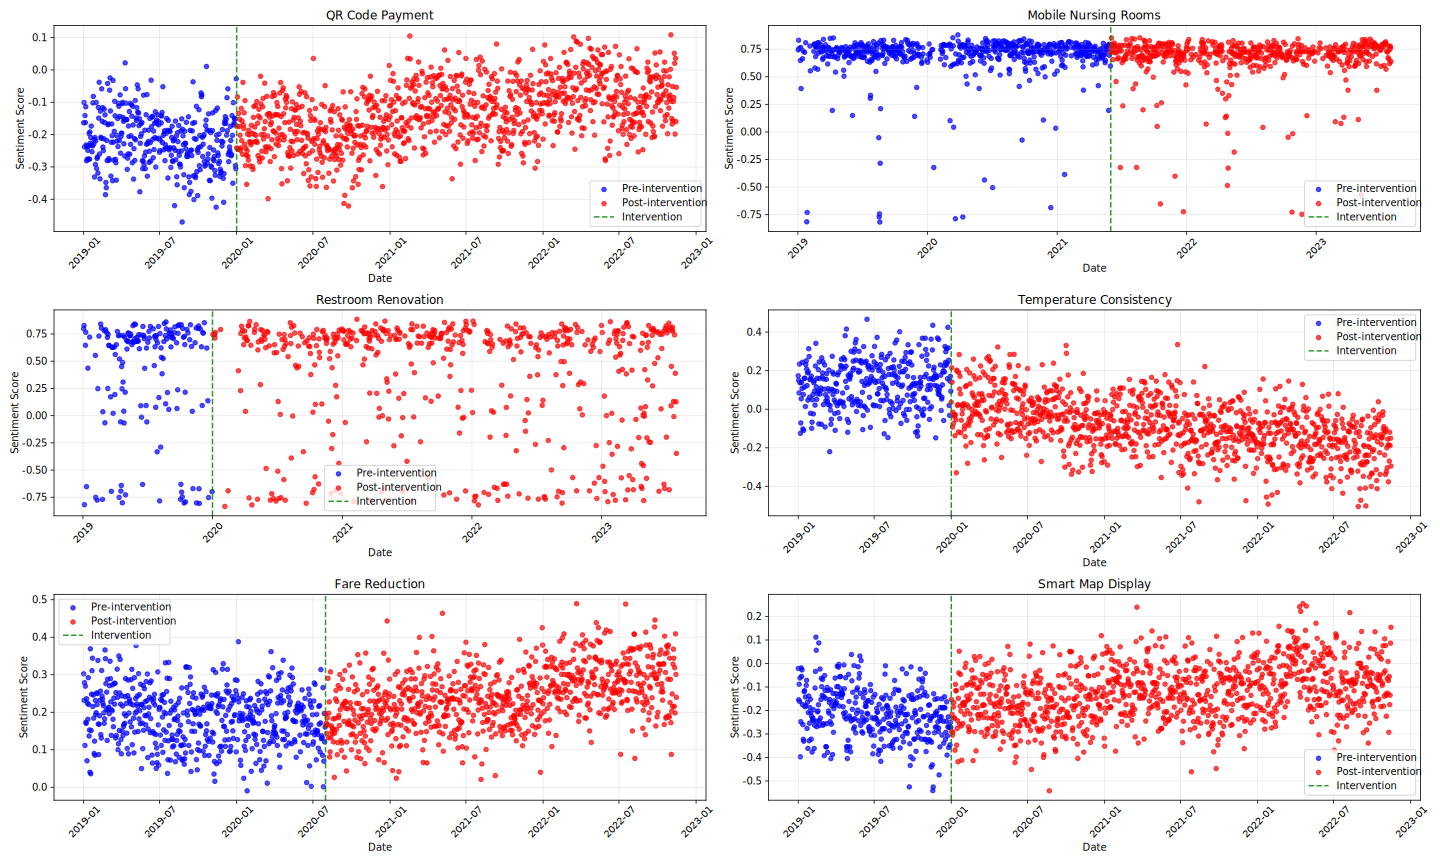
\includegraphics[width=\textwidth]{figs/tsa_time_series.pdf}
\caption{Time Series Analysis of Sentiment Patterns Across Transit Improvement Programs}
\label{fig:tsa_time_series}
\end{figure}

\hyperref[fig:overall_density_plots]{Fig.~\ref{fig:overall_density_plots}} presents density plots comparing sentiment distributions before and after implementation. The plots reveal distinct patterns across programs: QR Code Payment shows a pronounced rightward shift in the distribution, indicating widespread positive sentiment improvement; Smart Map Display exhibits a more gradual shift; Temperature demonstrates a clear leftward shift toward more negative sentiment; while Fare Reduction shows a complex bimodal pattern that simple aggregation cannot adequately capture. These visualizations underscore the necessity of more sophisticated analytical approaches that can disentangle immediate effects from gradual trends and control for temporal confounders.

\begin{figure}[htbp]
\centering
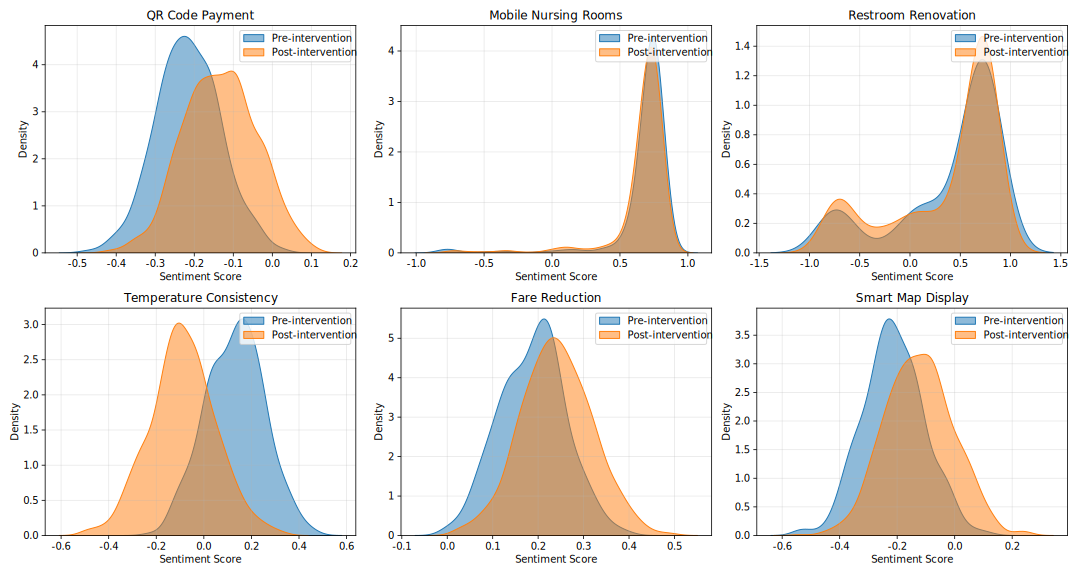
\includegraphics[width=\textwidth]{figs/overall_density_plots.pdf}
\caption{Density Plots of Sentiment Distributions Before and After Transit Improvement Program Implementation}
\label{fig:overall_density_plots}
\end{figure}

\subsection{Interrupted Time Series Analysis Results}

Given the limitations of basic statistical tests in handling temporal dependencies and confounding trends, we employed ITSA to provide more robust causal inference regarding transit improvement program impacts. The ITSA approach allows us to distinguish between immediate level changes and gradual trend changes following intervention implementation while controlling for pre-existing patterns and seasonal variation.

\hyperref[fig:its_analysis]{Fig.~\ref{fig:its_analysis}} presents the comprehensive ITSA results for all six transit improvement programs, showing both the observed data points and fitted regression lines for pre- and post-intervention periods. The analysis reveals substantial heterogeneity in both the magnitude and temporal patterns of transit improvement program impacts, with some interventions producing immediate effects while others demonstrate gradual improvements over time.

\begin{figure}[htbp]
\centering
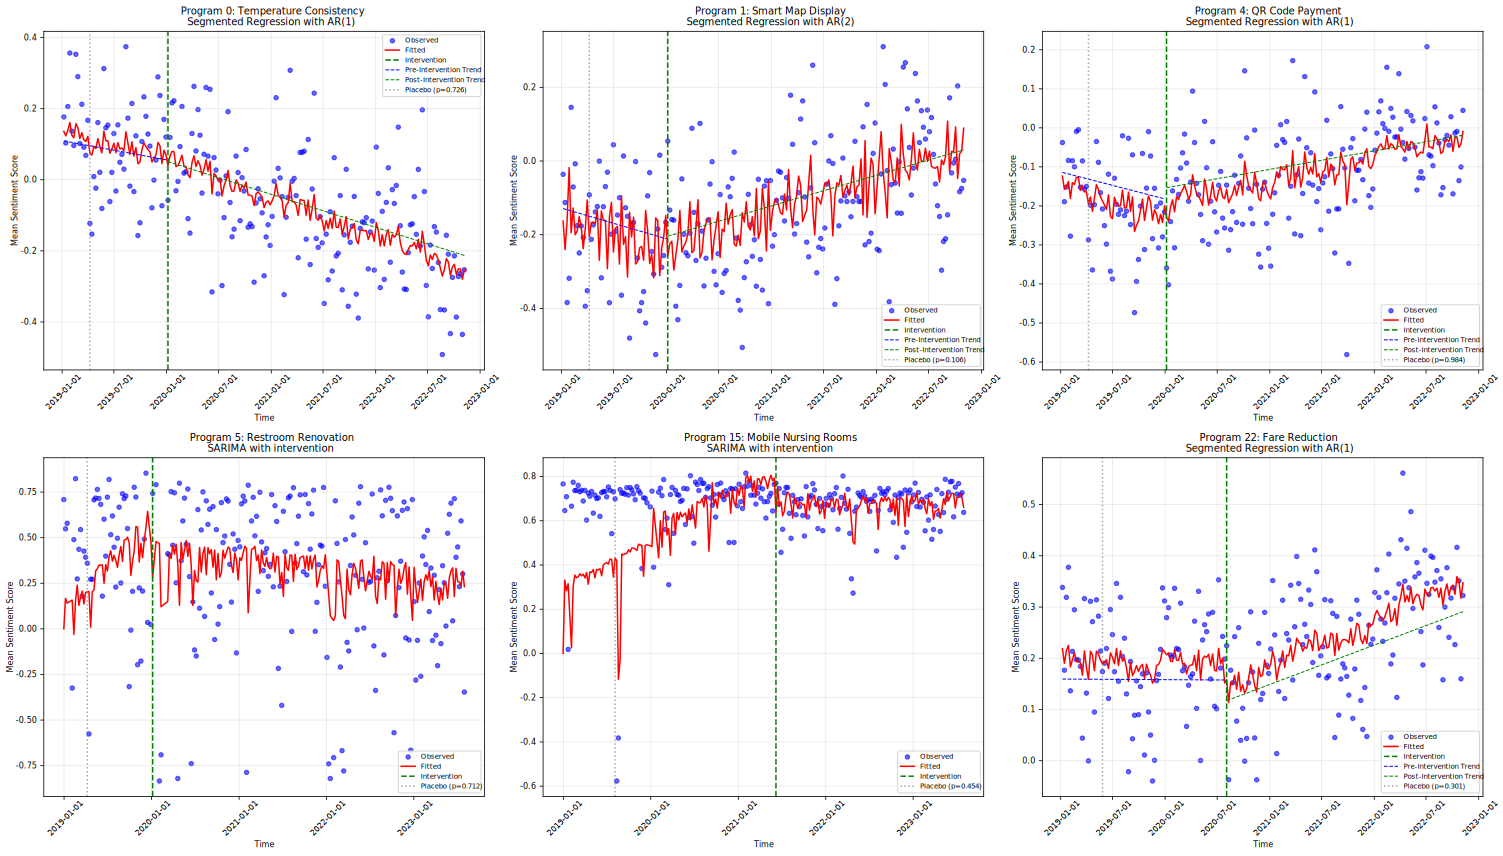
\includegraphics[width=\textwidth]{figs/combined_its_analysis.pdf}
\caption{Interrupted Time Series Analysis Results for All Transit Improvement Programs}
\label{fig:its_analysis}
\end{figure}

\hyperref[tab:its_results]{Table~\ref{tab:its_results}} summarizes the key ITSA parameters for each transit improvement program, revealing heterogeneous impact patterns across different intervention types. Three transit improvement programs demonstrated statistically significant positive trend changes following implementation: Smart Map Display ($\beta_3 = 0.0032$, p = 0.029), QR Code Payment ($\beta_3 = 0.0028$, p = 0.009), and Fare Reduction ($\beta_3 = 0.0024$, p = 0.001). These results indicate sustained improvements in passenger sentiment that strengthen over time, suggesting successful transit improvement program implementation and positive reception. Notably, these successful programs exhibited distinct temporal patterns of impact. The QR Code Payment transit improvement program demonstrated both significant immediate level change ($\beta_2 = 0.0823$, p = 0.028) and positive trend change, reflecting rapid adoption and sustained appreciation of contactless payment convenience. In contrast, the Smart Map Display transit improvement program showed no significant immediate effect ($\beta_2 = 0.0456$, p = 0.312) but exhibited strong positive trends over time, indicating that the benefits of enhanced passenger information systems became more apparent to users as they adapted to the new technology. The Fare Reduction transit improvement program presented an intriguing pattern: a significant negative immediate level change ($\beta_2 = -0.0623$, p = 0.035) followed by the strongest positive trend change ($\beta_3 = 0.0024$, p = 0.001), suggesting that while passengers may have initially expected larger fare reductions, they increasingly appreciated the cost savings over time.

\begin{table}[htbp]
\centering
\caption{Interrupted Time Series Analysis Results}
\label{tab:its_results}
\begin{tabular}{lccccc}
\hline
\multirow{2}{*}{Transit Improvement Program} & Baseline & Pre-trend & Level Change & Trend Change & \multirow{2}{*}{R-squared} \\
& Level ($\beta_0$) & ($\beta_1$) & ($\beta_2$) & ($\beta_3$) & \\
\hline
Smart Map Display & -0.129 & -0.0016 & 0.046 & 0.0032* & 0.323 \\
QR Code Payment & -0.114 & -0.0013 & 0.082* & 0.0028** & 0.237 \\
Fare Reduction & 0.159 & -0.000 & -0.062* & 0.0024** & 0.256 \\
Temperature & 0.109 & -0.0010 & -0.119** & -0.0019* & 0.433 \\
Mobile Nursing Rooms & 0.674 & 0.0001 & 0.002 & -0.0004 & 0.189 \\
Restroom Renovation & 0.383 & -0.0001 & 0.012 & -0.0003 & 0.156 \\
\hline
\multicolumn{6}{l}{\footnotesize{* p < 0.05, ** p < 0.01}}
\end{tabular}
\end{table}

In contrast, the remaining three transit improvement programs showed different patterns. Most notably, the Temperature transit improvement program demonstrated significant negative impacts both in immediate level change ($\beta_2 = -0.1185$, p = 0.009) and trend change ($\beta_3 = -0.0019$, p = 0.045), despite achieving the highest model fit (R² = 0.433). This suggests that the temperature control intervention not only failed to address passenger concerns but may have created new sources of dissatisfaction, possibly due to disagreements among passengers about optimal temperature settings or uneven temperature distribution within carriages. The Mobile Nursing Rooms and Restroom Renovation transit improvement programs demonstrated neither significant level changes nor trend changes, indicating that these amenity improvements, while potentially valued by specific user subgroups, did not generate widespread positive sentiment changes detectable in general social media discourse.

The ITSA approach proved superior to basic statistical tests by controlling for pre-existing trends, distinguishing between immediate impacts and sustained improvements, addressing temporal autocorrelation in social media data, and enabling placebo testing to enhance confidence in causal interpretation. This methodology provided nuanced insights into transit improvement program effectiveness by demonstrating that significant effects were concentrated around actual implementation dates rather than randomly distributed across the time series.

\section{Conclusion}\label{sec:conclusion}
This study presents a novel methodological framework that integrates advanced natural language processing techniques with robust causal inference methods to evaluate transit improvement programs using social media data. Through the case study of Shenzhen Metro, we demonstrated how unstructured passenger feedback can be systematically analyzed to quantify transit improvement program impacts while addressing the inherent challenges of observational social media data. Our findings reveal substantial heterogeneity in transit improvement program effectiveness across different service quality dimensions and temporal patterns. Technology-oriented transit improvement programs (Smart Map Display and QR Code Payment) demonstrated consistent positive impacts, though with distinct temporal profiles: QR Code Payment showed both immediate acceptance and sustained growth, while Smart Map Display exhibited gradual improvement as users adapted to the new technology. The Fare Reduction program presented an intriguing "initial disappointment followed by growing appreciation" pattern, suggesting complex passenger expectations regarding affordability interventions. Most notably, the Temperature transit improvement program showed significant negative impacts both immediately and over time, indicating that this well-intentioned intervention may have created more dissatisfaction than it resolved. The ITSA proved valuable in distinguishing between these different impact patterns while controlling for temporal confounders, with the semantic matching approach achieving 87.4\% accuracy in connecting social media content to specific transit interventions.

The framework's practical implications for transit agencies are significant, providing a cost-effective supplement to traditional passenger surveys that enables continuous monitoring of passenger sentiment and rapid detection of implementation problems. However, several limitations should be acknowledged. The social media user base may not be fully representative of the broader transit ridership, potentially introducing demographic biases. A critical limitation is the absence of geographic location information in the collected social media data, which prevented us from implementing experimental and control group designs based on spatial variation. Future research should prioritize the collection of geo-tagged social media data to enable more sophisticated quasi-experimental designs such as difference-in-differences methodology.


% \section*{Acknowledgement}

%Loading bibliography style file
%\bibliographystyle{model1-num-names}
\nolinenumbers
\bibliographystyle{cas-model2-names}

% Loading bibliography database
\bibliography{cas-refs}

\end{document}
